\begin{pastexam}[label={px:ust-114-ee-ds-28}]{臺聯大電機類 114 學年度 問答題第 4 題}
（問答；10 分）

Based on the following codes, please answer the questions below:
\begin{enumerate}[label=(\Alph*)]
\item What is the tree structure in the code? (3 points)
\item What is the output of the code? (3points)
\item In the zigzagLevelOrder method, if the initial value of leftToRight is changed to false, what
will the output be after execution? Please provide a detailed explanation. (4 points)
\end{enumerate}

\begin{minted}[fontsize=\small]{text}
Class TreeNode
    Attributes: value, left, right

    Constructor(value):
        value = value
        left = null
        right = null

Function zigzagLevelOrder(root):
    result = empty list of lists
    If root is null:
        Return result

    queue = empty queue
    Enqueue(root, queue)
    leftToRight = true

    While queue is not empty:
        levelSize = size of queue
        currentLevel = empty list

        For i = 0 to levelSize - 1:
            currentNode = Dequeue(queue)

            If leftToRight:
                Append(currentNode.value, currentLevel)
            Else:
                Insert at beginning(currentNode.value, currentLevel)

            If currentNode.left is not null:
                Enqueue(currentNode.left, queue)
            If currentNode.right is not null:
                Enqueue(currentNode.right, queue)

        Append(currentLevel, result)
        leftToRight = not leftToRight

    Return result

Function main:
    root = new TreeNode(1)
    root.left = new TreeNode(2)
    root.right = new TreeNode(3)
    root.left.left = new TreeNode(4)
    root.left.right = new TreeNode(5)
    root.right.right = new TreeNode(6)

    result = zigzagLevelOrder(root)
    Print(result)
\end{minted}
\end{pastexam}

\begin{pastsoln}
\textbf{(A)} 依 main 建出的二元樹：根 1；1 的左子節點 2、右子節點 3；2 的左、右子節點是 4、5；3 只有右子
節點 6。
\begin{center}
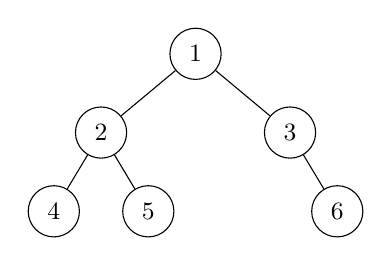
\begin{tikzpicture}[every node/.style={circle,draw,minimum size=6.5mm,inner sep=0pt,font=\small},
  level distance=10mm, level 1/.style={sibling distance=24mm}, level 2/.style={sibling distance=12mm}]
\node {1}
  child {node {2} child {node {4}} child {node {5}}}
  child {node {3} child[missing] child {node {6}}};
\end{tikzpicture}
\end{center}

\textbf{(B)} 這是用佇列做的層序走訪（資結書第~7.3.2~節）：每一輪先記下佇列長度 levelSize，正好把同一層的
節點全部取出，子節點則依「左、右」的順序排進佇列給下一層。 同一層的節點總是由左到右取出；
leftToRight 為真時把值接在 currentLevel 尾端（由左到右），為假時插在開頭（結果反過來，由右到左）。
每處理完一層就把 leftToRight 反過來。
\begin{center}
\small
\begin{tabular}{cclll}
\toprule
層 & leftToRight & 取出順序 & currentLevel & 佇列（處理完這層） \\
\midrule
0 & true & 1 & [1] & 2, 3 \\
1 & false & 2, 3 & 2 $\to$ [2]；3 插開頭 $\to$ [3, 2] & 4, 5, 6 \\
2 & true & 4, 5, 6 & [4, 5, 6] & 空 \\
\bottomrule
\end{tabular}
\end{center}
輸出 \texttt{[[1], [3, 2], [4, 5, 6]]}：第一層由左到右，第二層由右到左，第三層又由左到右，呈之字形。

\textbf{(C)} 初值改成 false，只有方向從第 0 層開始就反過來；取出順序和佇列的內容完全不變（子節點一律先左
後右排進佇列，與 leftToRight 無關）。
\begin{itemize}
\item 第 0 層（false）：[1]（一個元素，方向沒差）。
\item 第 1 層（true）：依取出順序接在尾端，[2, 3]。
\item 第 2 層（false）：取出 4、5、6，每次插在開頭：[4] $\to$ [5, 4] $\to$ [6, 5, 4]。
\end{itemize}
輸出 \texttt{[[1], [2, 3], [6, 5, 4]]}：變成第 0 層之後「先由左到右、再由右到左」的之字形，每一層的
方向都和 (B) 相反。

複雜度：每個節點進出佇列各一次，時間 $O(n)$；不過「插在開頭」若用陣列實作，每次要搬移
$O(\text{該層大小})$，最壞會變成 $O(n^2)$，實作時改用雙端佇列或先收集再反轉即可維持 $O(n)$。
\end{pastsoln}
